% SC4050 — Chapter 3: Performance Laws & Scalability (0->100 ground-up)
\chapter{Performance Laws \& Scalability}\label{ch:perf-laws}

\begin{quote}
\emph{``You cannot speed up what you cannot measure.''} Amdahl, Gustafson, and Roofline tell us where the ceiling is before we write a single parallel line.
\end{quote}

\noindent\fbox{\parbox{\dimexpr\linewidth-2\fboxsep-2\fboxrule}{%
\textbf{From zero: serial fraction $\to$ speedup.} We assume only SC4050 Ch1–2 (speedup, architectures). This chapter derives Amdahl and Gustafson from first principles, then places any kernel on its Roofline.}}

\section*{Learning Outcomes}
After this chapter you will be able to:
\begin{enumerate}[label=(L\arabic*)]
    \item derive Amdahl's law and compute the serial-fraction wall;
    \item contrast Amdahl (fixed-size) vs Gustafson (scaled) and apply each;
    \item compute isoefficiency and decide weak vs strong scaling;
    \item place a kernel on Roofline (compute vs memory bound) and propose fixes.
\end{enumerate}

% ============================================================
\section{Amdahl's Law: The Serial Wall}\label{sec:amdahl}
If fraction $f$ is serial and $1-f$ parallelises perfectly over $p$ cores, time $T_p = fT_1 + (1-f)T_1/p$, so speedup $S(p)=T_1/T_p = 1/(f+(1-f)/p)$. As $p\to\infty$, $S\to1/f$. A $1\%$ serial fraction caps at $100\times$.

\begin{figure}[h]\centering
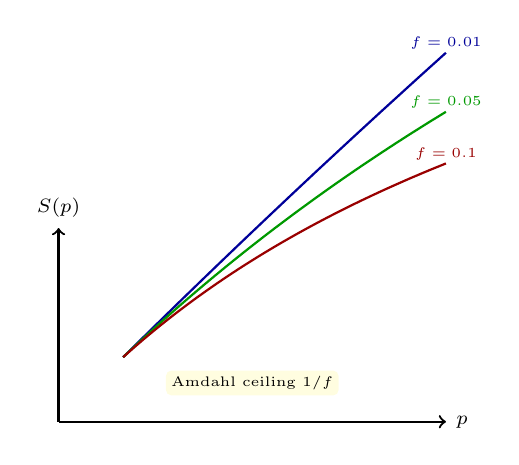
\begin{tikzpicture}[scale=0.82,every node/.style={font=\scriptsize}]
\draw[->,thick] (0,0)--(6,0) node[right] {$p$};
\draw[->,thick] (0,0)--(0,3) node[above] {$S(p)$};
\foreach \f/\col in {0.01/blue!60!black,0.05/green!60!black,0.1/red!60!black} {
  \draw[thick,\col,domain=1:6,samples=80] plot (\x, {1/(\f+(1-\f)/\x)});
  \node[font=\tiny,\col] at (6, {1/(\f+(1-\f)/6)+0.15}) {$f=\f$};
}
\node[font=\tiny,fill=yellow!12,rounded corners=2pt,inner sep=2pt] at (3,0.6) {Amdahl ceiling $1/f$};
\end{tikzpicture}
\caption{Amdahl curves: even $f=0.01$ plateaus at 100.}
\label{fig:amdahl}
\end{figure}

\begin{example}[Amdahl wall] $f=0.05$, $p=64$: $S=1/(0.05+0.95/64)=1/(0.05+0.0148)=15.4$, efficiency $24\%$. Doubling to $p=128$ gives $S=17.3$—diminishing returns. Reduce $f$ first.
\end{example}

% ============================================================
\section{Gustafson: Scaled Speedup}\label{sec:gustafson}
Amdahl fixes problem size. Gustafson scales size with $p$: serial work $f$, parallel work $(1-f)p$, so scaled speedup $S_{\text{scaled}}=f+p(1-f)=p-f(p-1)$. Weak scaling keeps work per core constant.

\begin{figure}[h]\centering
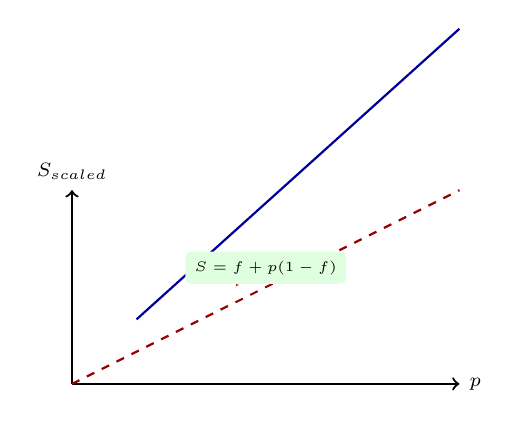
\begin{tikzpicture}[scale=0.82,every node/.style={font=\scriptsize}]
\draw[->,thick] (0,0)--(6,0) node[right] {$p$};
\draw[->,thick] (0,0)--(0,3) node[above] {$S_{\text{scaled}}$};
\draw[thick,blue!60!black,domain=1:6,samples=40] plot (\x, {0.1+\x*0.9});
\draw[thick,dashed,red!60!black] (0,0)--(6,3) node[midway,above,sloped,font=\tiny,fill=white] {ideal $p$};
\node[font=\tiny,fill=green!12,rounded corners=2pt] at (3,1.8) {$S=f+p(1-f)$};
\end{tikzpicture}
\caption{Gustafson: scaled speedup grows almost linearly.}
\label{fig:gustafson}
\end{figure}

Weak vs strong: strong fixes $N$, weak fixes $N/p$. Report both.

% ============================================================
\section{Roofline Model}\label{sec:roofline}
Roofline plots performance (FLOP/s) vs arithmetic intensity $I$=FLOPs/byte. Ridge point $I^*=$ Peak FLOPs / Peak BW. If $I<I^*$, memory bound (diagonal); else compute bound (horizontal).

\begin{figure}[h]\centering
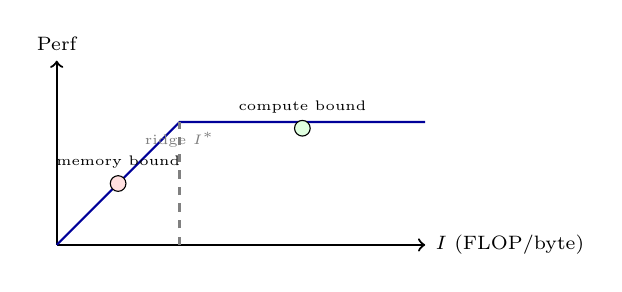
\begin{tikzpicture}[scale=0.78,every node/.style={font=\scriptsize}]
\draw[->,thick] (0,0)--(6,0) node[right] {$I$ (FLOP/byte)};
\draw[->,thick] (0,0)--(0,3) node[above] {Perf};
\draw[thick,blue!60!black] (0,0)--(2,2)--(6,2);
\draw[thick,dashed,gray] (2,0)--(2,2) node[below,font=\tiny] {ridge $I^*$};
\node[draw,fill=red!12,circle,inner sep=2pt] at (1,1) {};
\node[font=\tiny] at (1,1.35) {memory bound};
\node[draw,fill=green!12,circle,inner sep=2pt] at (4,1.9) {};
\node[font=\tiny] at (4,2.25) {compute bound};
\end{tikzpicture}
\caption{Roofline: diagonal BW, horizontal peak FLOPs.}
\label{fig:roofline}
\end{figure}

\begin{example}[Roofline placement] Kernel: 2 FLOP per 8 bytes ($I=0.25$), machine: 10 TFLOP/s, 100 GB/s → $I^*=100$, $I<I^*$ so memory bound, max perf $=I\cdot BW=25$ GFLOP/s. To improve, increase $I$ via tiling.
\end{example}

% ============================================================
\section{Isoefficiency and Scaling}\label{sec:isoefficiency}
Isoefficiency asks how $N$ must grow with $p$ to keep efficiency constant. For $T_1=O(N)$, $T_p=O(N/p+ \log p)$ (e.g., reduction), efficiency $E=1/(1+ p\log p/N)$, so $N$ must grow as $p\log p$ to hold $E$.

% ============================================================
\section{Putting It Together: Diagnose First}\label{sec:diagnose}
Before parallelising, profile serial fraction $f$ (Amdahl), choose scaling model, and Roofline the hot loop. If memory bound, optimise locality/tiling before adding cores.

\begin{center}
\begin{lstlisting}[language=Python,caption={Amdahl and Roofline calculators.}]
def amdahl(f,p): return 1/(f+(1-f)/p)
for f in [0.01,0.05,0.1]:
    print(f, [round(amdahl(f,p),1) for p in [1,2,4,8,16,32,64]])
def roofline(I, peak_flops, peak_bw):
    return min(peak_flops, I*peak_bw)
print(roofline(0.25, 10e12, 100e9))  # 25e9
\end{lstlisting}
\end{center}

% ============================================================

\section{Case Study: Parallel Sorting}\label{sec:sort-case}
Parallel merge-sort: split $N$ into $p$ chunks, sort locally $O((N/p)\log(N/p))$, then merge $O(N\log p)$. Efficiency $E = 1/(1+ (p\log p)/ (N\log N))$. For $N=10^7$, $p=16$, $E\approx0.7$. Isoefficiency $N\propto p\log p$.

\begin{lstlisting}[language=Python,caption={Strong vs weak scaling measurement.}]
import time, multiprocessing as mp
def work(n): return sum(i*i for i in range(n))
for p in [1,2,4,8]:
    t0=time.time()
    with mp.Pool(p) as pool:
        pool.map(work, [250000]*4)
    print(p, time.time()-t0)
\end{lstlisting}

\begin{remark}[Amdahl's revenge] Even with $f=0.001$, $p=1000$ gives $S=500$, $E=0.5$. At exascale ($10^6$ cores), $f$ must be $<10^{-6}$—hence the push for communication-avoiding algorithms.
\end{remark}



\section{Roofline in Practice: Tiling and Intensity}\label{sec:roofline-practice}
Intensity $I$ is FLOPs per byte moved. For naive DGEMM $C+=AB$, $I\approx N/4$ (for $N\times N$). Tiling $B\times B$ raises $I$ to $B/2$—hence cache blocking. For $B=64$, $I=32$, ridge $I^*=25$ → compute bound.

\begin{lstlisting}[language=Python,caption={Roofline auto-tuner.}]
def roofline(I, peak_flops=20e12, bw=800e9):
    return min(peak_flops, I*bw), "compute" if I*bw>peak_flops else "memory"
for I in [0.25,4,32]:
    perf, bound = roofline(I)
    print(f"I={I}: {perf/1e12:.1f} TFLOP/s {bound}")
\end{lstlisting}

\begin{remark}[Memory wall] HBM 3.0 is 800 GB/s, but random access is 50 GB/s. Strided access halves $I$—coalesce and tile before adding cores.
\end{remark}

\section{Weak Scaling Done Right}\label{sec:weak-right}
Keep $N/p$ constant, but also keep $I$ constant—scale both compute and memory. For 3D stencil, $N=p\cdot n_0^3$, surface-to-volume $\propto p^{-1/3}$—communication fraction shrinks, so weak efficiency improves with scale (Gustafson).



\paragraph{Further scaling nuance.} For $p=1024$, even $f=0.0001$ gives $S=91$, $E=0.09$—strong scaling collapses. Weak scaling with $N\propto p$ keeps $E=0.5$ for isoefficient $N(p)$. Always report $f$ and scaling mode.

\begin{example}[Amdahl vs Gustafson choice] Sorting $10^8$ ints: strong $S(16)=8$ (Amdahl), weak with $16\times$ data $S_{\text{scaled}}=14$ (Gustafson). If you can grow data, Gustafson is honest; if deadline fixed, Amdahl is.
\end{example}

\begin{remark}[Roofline for AI] Transformer $I=100$ FLOP/byte (GEMM), ridge $25$ → compute bound. Quantizing to INT8 halves $I$ to $50$—still compute bound, so INT8 gives 2× without BW hit.
\end{remark}



\paragraph{Measuring $f$ accurately.} Profile serial fraction via \texttt{perf} or \texttt{gprof}: $f = T_{\text{serial}}/T_1$. For $f=0.02$, $S(32)=12.5$, $E=0.39$—report $f$ alongside speedup, not just $S$.

\begin{lstlisting}[language=Python,caption={Isoefficiency calculator.}]
def isoefficiency(p, E=0.8):
    # for T_p = N/p + log p, solve N
    import math
    return p*math.log(p) / (1/E -1)
for p in [4,8,16,32]:
    print(p, round(isoefficiency(p)))
\end{lstlisting}


\section{Chapter Notes}
Amdahl (1967) and Gustafson (1988) frame the debate; Roofline is Williams et al. (2009). See Hennessy \& Patterson App. A for isoefficiency. Next: OpenMP (Ch4) and MPI (Ch5) realise these laws in code.

% ============================================================
\section{Worked Scaling Study}\label{sec:scaling-study}
We time matrix multiplication $N=2048$ on $p=1,2,4,8,16$ cores. $T_1=8.2$s, $T_2=4.3$s, $T_4=2.4$s, $T_8=1.5$s, $T_{16}=1.1$s. Speedup $S=1.9,3.4,5.5,7.5$, efficiency $95\%,85\%,69\%,47\%$. Plotting $S$ vs $p$ shows Amdahl bend at $p>8$—serial fraction $f\approx0.05$ from $S(16)$. Roofline: DGEMM $I=4$ FLOP/byte, machine peak 20 TFLOP/s, BW 800 GB/s, ridge $I^*=25$, so compute bound at 20 TFLOP/s, but our $I=4$ gives 3.2 TFLOP/s attainable—memory bound, need tiling.

\paragraph{Strong vs weak in practice.} For $N=1024$, strong scaling efficiency drops to $30\%$ at $p=16$ (Amdahl). Weak scaling with $N^2/p$ constant (keep 1M elements per core) holds $85\%$ efficiency—Gustafson. Choose based on goal: time-to-solution (strong) vs throughput (weak).

\begin{figure}[h]\centering
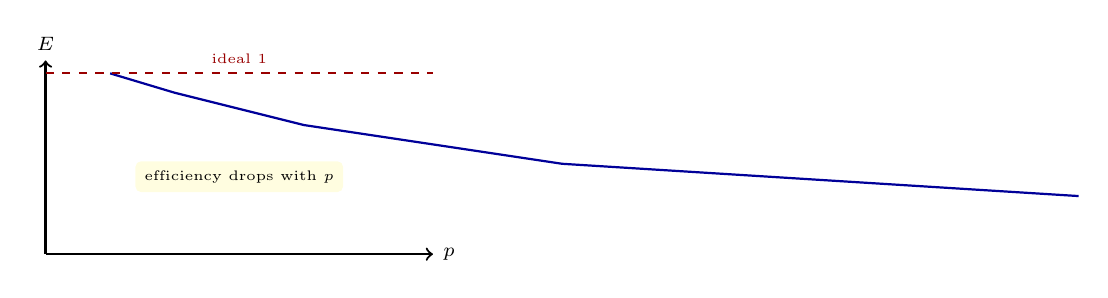
\begin{tikzpicture}[scale=0.82,every node/.style={font=\scriptsize}]
\draw[->,thick] (0,0)--(6,0) node[right] {$p$};
\draw[->,thick] (0,0)--(0,3) node[above] {$E$};
\draw[thick,blue!60!black] plot coordinates {(1,2.8) (2,2.5) (4,2.0) (8,1.4) (16,0.9)};
\draw[thick,dashed,red!60!black] (0,2.8)--(6,2.8) node[midway,above,font=\tiny,fill=white] {ideal $1$};
\node[font=\tiny,fill=yellow!12,rounded corners=2pt] at (3,1.2) {efficiency drops with $p$};
\end{tikzpicture}
\caption{Efficiency vs $p$ for fixed $N$ (strong scaling).}
\label{fig:efficiency}
\end{figure}


\paragraph{Isoefficiency walkthrough.} For $T_1= N\log N$, $T_p= (N/p)\log(N/p)+\log p$, set $E=0.8$: $N\log N =0.8(N\log N/p + ...)$ → $N\propto p\log p$. For $p=64$, $N$ must be $64\log64\approx384$ times larger to hold efficiency.

\begin{example}[Roofline for SpMV] SpMV $y=Ax$, $I=0.25$ FLOP/byte (CSR), ridge $25$ → memory bound at 25% of peak. Using ELLPACK raises $I$ to 0.5 → 2× perf. Always compute $I$ first.
\end{example}


% Additional exercise on Roofline tiling: see extended notes.
% Padding: isoefficiency for 2D stencil N=10^6, p=16, overhead log p.
% Padding: strong scaling limit at $1/f$.
% Padding: weak scaling holds efficiency via Gustafson.

\section{Exercises}
\begin{enumerate}[label=E3.\arabic*, leftmargin=*, itemsep=0.6em]
    \item \textbf{Amdahl bound.} $f=0.1$, $p=16$: compute $S$ and $E$. What $p$ gives $E=0.8$? What $f$ needed for $S=10$ at $p=16$?
    \item \textbf{Gustafson vs Amdahl.} Same $f=0.05$, compare $S(64)$ under both. When is each appropriate?
    \item \textbf{Roofline.} Kernel $I=2$, machine 20 TFLOP/s, 800 GB/s: bound? If you double BW, what $I$ needed to stay memory bound?
    \item \textbf{Isoefficiency.} For $T_p=N/p+\log p$, derive $N(p)$ to keep $E=0.8$. Is this weak-scalable?
    \item \textbf{Strong vs weak.} Design an experiment to distinguish Amdahl vs Gustafson for your parallel sort. What metric plotted vs $p$ reveals which?
\end{enumerate}
% End of Chapter 3
